%%%%%%%%%%%%%%%%%%%%%%%%%%%%%%%%%%%%%%%%%%%%%%%%%%%%%%%%%%%%%%%%%%%%%%%%
\begin{frame}[t]{[LF63, UF64] Sound Mode - Punk}
\begin{tiny}
\begin{tabular}{@{}lccc@{}}
\toprule
Function & Off/On & Option & Specification \\
\midrule
Audio EQ & \color{black}{Off} & Instart &
\multirow{10}{60mm}{
\begin{itemize}
\item Frequency Response Check
	\begin{itemize}
	\item 80Hz에서 ref 신호와의 레벨 차이값이 7.0±1dBr 이내
	\item 200Hz에서 ref 신호와의 레벨 차이값이 5.5±1dBr 이내
	\item 1kHz에서 ref 신호와의 레벨 차이값이 7.5±1dBr 이내
	\item 4kHz에서 ref 신호와의 레벨 차이값이 5.0±1dBr 이내
	\item 8kHz에서 ref 신호와의 레벨 차이값이 7.0±1dBr 이내
	\end{itemize}
\end{itemize}
} \\
Sound Engine & \color{blue}{On} & Instart & \\
Clearvoice & \color{black}{Off} & & \\
Autovolume & \color{black}{Off} & & \\
Surround & \color{black}{Off} & & \\
Smart Sound & \color{black}{Off} & & \\
3D Sound Zooming & \color{black}{Off} & & \\
Sound Mode & \color{blue}{On} & \color{blue}{Punk} & \\
Sound Optimizer & \color{black}{Off} & & \\
OSD Volume & \color{blue}{On} & Vol.40 & \\
\midrule
\end{tabular}
\end{tiny}

\begin{figure}[b]
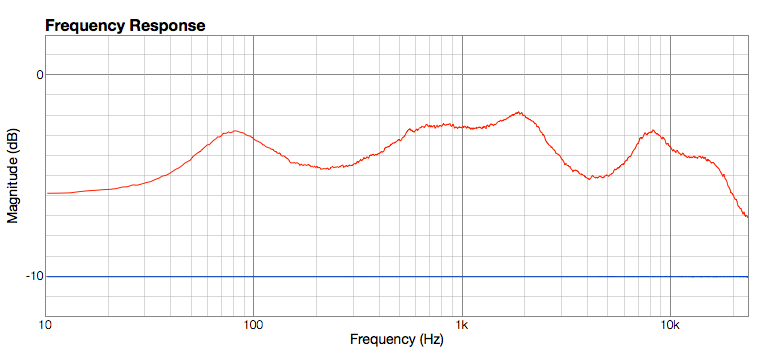
\includegraphics[height=0.4\textwidth]{figures/punk.png}
\end{figure}

\end{frame}
